\documentclass[a4paper,francais,titlepage]{article}
\usepackage[utf8x]{inputenc}  
%% utf8x support des espaces insécables ' ' au lieu da la macro ~)

\usepackage[T1]{fontenc}
\usepackage[francais]{babel}
\usepackage{latexsym}
\usepackage{url}
\usepackage{graphicx}
\usepackage{enumerate}
\usepackage{lscape}   %% pour le mode paysage \begin{landscape}
\usepackage{hyperref}
\hypersetup{
    colorlinks,
    citecolor=black,
    filecolor=black,
    linkcolor=black,
    urlcolor=black
}

% continuité numérotation figures
\usepackage{chngcntr} 

% style général
\usepackage{vmargin}

\setmarginsrb{2.5cm}{2cm}{2.5cm}{1cm}{0.5cm}{1.5cm}{2cm}{2cm}
%1 est la marge gauche
%2 est la marge en haut
%3 est la marge droite
%4 est la marge en bas
%5 fixe la hauteur de l'entête
%6 fixe la distance entre l'entête et le texte
%7 fixe la hauteur du pied de page
%8 fixe la distance entre le texte et le pied de page

%%ressources
\graphicspath{{../ressources/}}

\begin{document}

%%%%%%%%% Première page: titre
\begin{titlepage}
 \begin{center}
	\vspace*{3.5cm}
	\Large \textbf{Gifts4YourFriends} \\
	\vspace{0.2cm}
	\small Rapport
	\vspace{2cm}

	\huge \textbf{Nuit de l'informatique} \\
	\vspace{0.3cm}
	\large {Défi Akka Technologies}
	\vspace{1.5cm}
 \end{center}
 
 \begin{flushleft}
	\normalsize {\hspace{6cm}Responsables de l'événement: \\ 
				 \hspace{7.0cm} Blanc Xavier \\
				 \hspace{6.7cm} Bromberg David \\
				 \hspace{6.6cm} Fleury Emmanuel}
	\vspace{2cm}
 \end{flushleft}
 
   \begin{center}
   
\includegraphics[scale=0.3]{logo_bx1.jpg}
   	\vfill 
   	\vspace{2cm}
	\normalsize {Rage Against The Turing Machine\\}
	\vspace{1.5cm} 
	{\today}.
 \end{center}
\end{titlepage}
%%%%%%%% Fin première page

\section{Introduction : Choix de la méthode}
Dès la proposition des sujets, nous avions en tête de mettre en pratique les cours de certains membres du groupe en Conduite de Projet, et d'ainsi utiliser les méthodes Agiles et SCRUM. Nous avons donc au préalable désigné 2 SCRUM-Masters et réparti l'équipe en 4 sous-équipes. Ensuite au lancement de l'événement, nous avons effectué un BrainStorming pour définir les objectifs exacts puis les backlogs. Finalement les 3 sprints de 3h30 ont pu démarrer. Nous nous sommes servi de git en gestionnaire de version pour les défis, bien qu'il nous a posé pas mal de problème à chaque push.

\subsection*{Les informations}
\subparagraph{}Nous trouvant dans la même classe, la catégorie d'information la plus facile à mettre en œuvre était la communication. Dans ce cas, rien ne vaut le dialogue direct avec les autres membres de l'équipe. Nous ne nous sommes donc pas trop appliqué sur les messages de commit et n'avons dès lors utilisé notre googlegroup que pour envoyer le lien du repository git. Le tableau a été d'une grande utilisé quant aux informations persistantes à faire passer telles que le plan des sprints, les logs de Twitter et certaines commandes.

\subparagraph{}Nous étions divisés en 4 équipes, la première faisant le serveur, la deuxième le web services, et les deux dernières les GUI WP7 et Android. Chaque équipe se débrouillait comme il était nécessaire à l'instant: programmation en binôme, trinôme ou en solo, se basant sur leurs connaissances ou sur des recherches dans . A partir de 5h, les membres des équipes ne pouvant contribuer activement sans risque de duplication se sont mis aux rapports.

\subparagraph{}Le but était de terminer tout les projets auxquels nous étions inscrit en 1 seul gros projet, et de faire fonctionner le tout avec des fonctionnalités simples sans, pour le moment, se soucier de la sécurité. Malheureusement à cause d'un blocage honteux, nous n'avons réussi qu'à avoir chaque parties mais indépendantes, sans être mises en communs. Il reste donc seulement à mettre en commun chaque partie.

\subparagraph{}En ce qui concerne le code, nous avons simplement utilisé la norme Java, sans vraiment se concerter, car nous trouvions cela secondaire.

\section{La méthode en image}
   	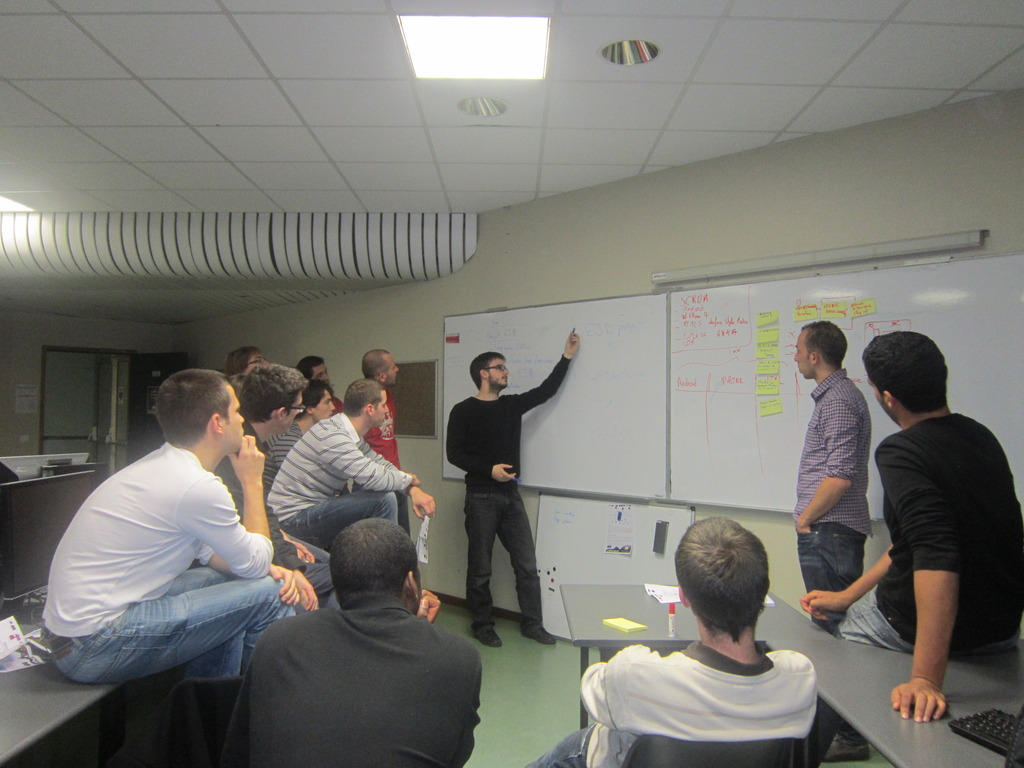
\includegraphics[scale=0.378]{brainstorming7.jpeg} \hspace{0.3cm} 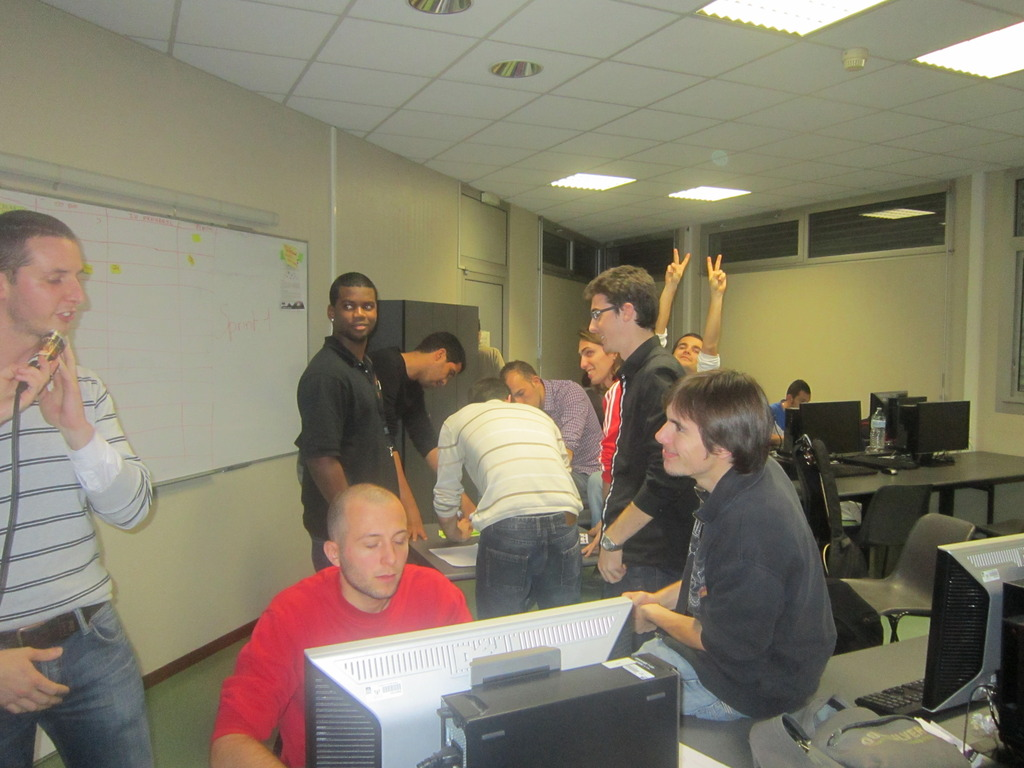
\includegraphics[scale=0.378]{brainstorming4.jpeg} \hspace{0.3cm} 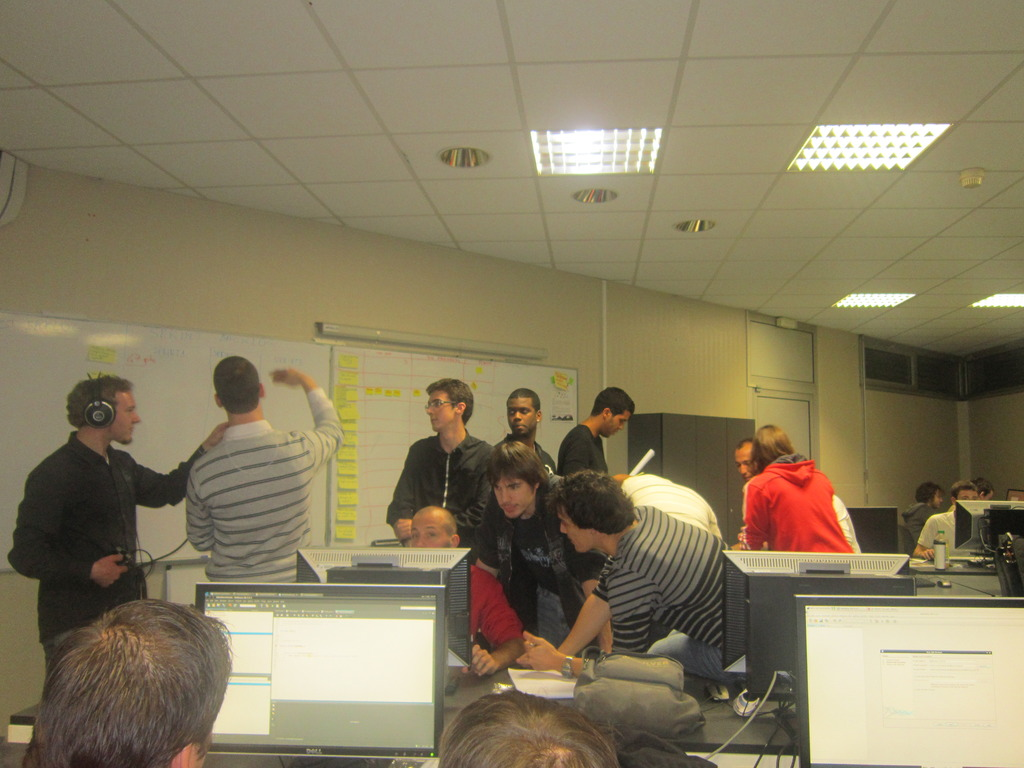
\includegraphics[scale=0.38]{brainstorming5.jpeg} \\
   	Le brainstorming du début avec création des backlogs, tout en se faisant interviewer par Radio Campus. \\
   
  	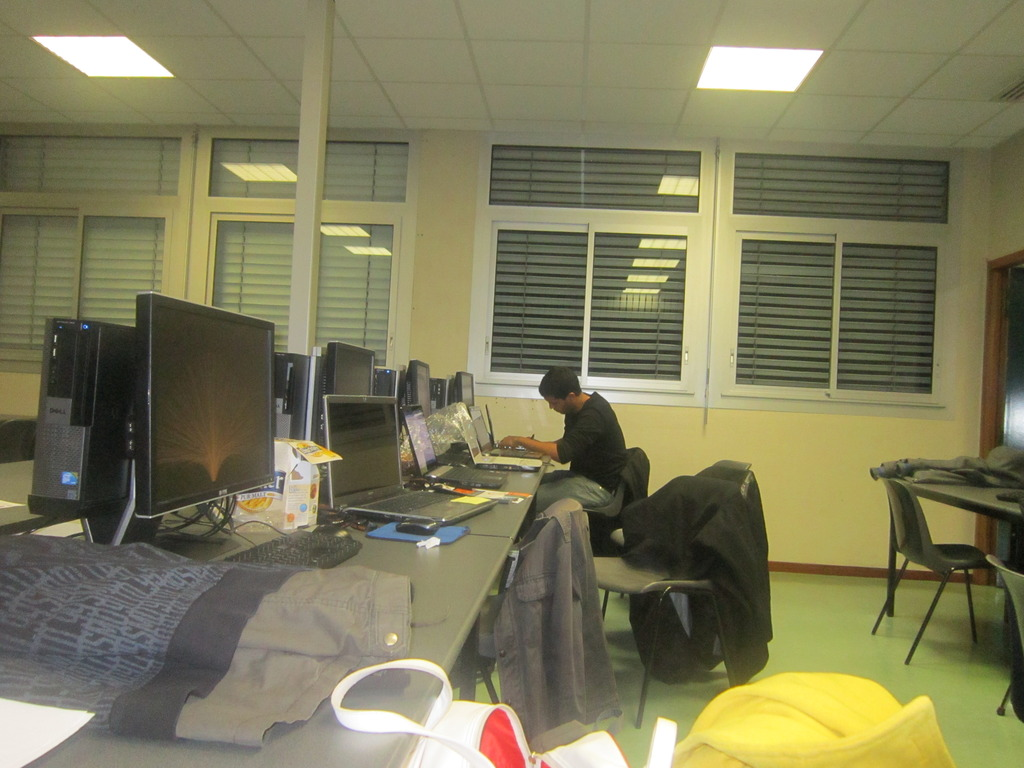
\includegraphics[scale=0.38]{solo.jpeg} \hspace{0.3cm} 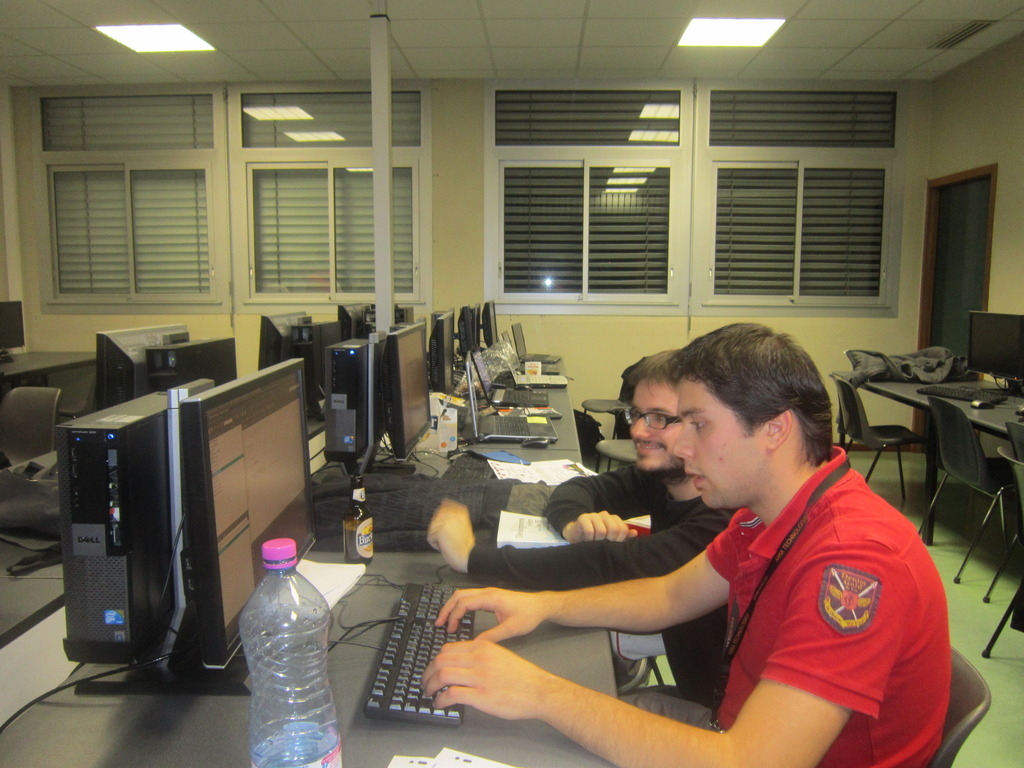
\includegraphics[scale=0.38]{binome.jpeg} \\
    Le travail se faisant ensuite par 3, 2 ou seul selon la difficulté et le type de la tâche. \\
    
    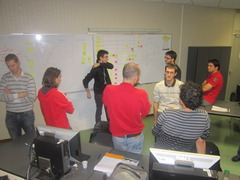
\includegraphics[scale=1.6]{brainstorming.jpeg} \hspace{0.3cm} 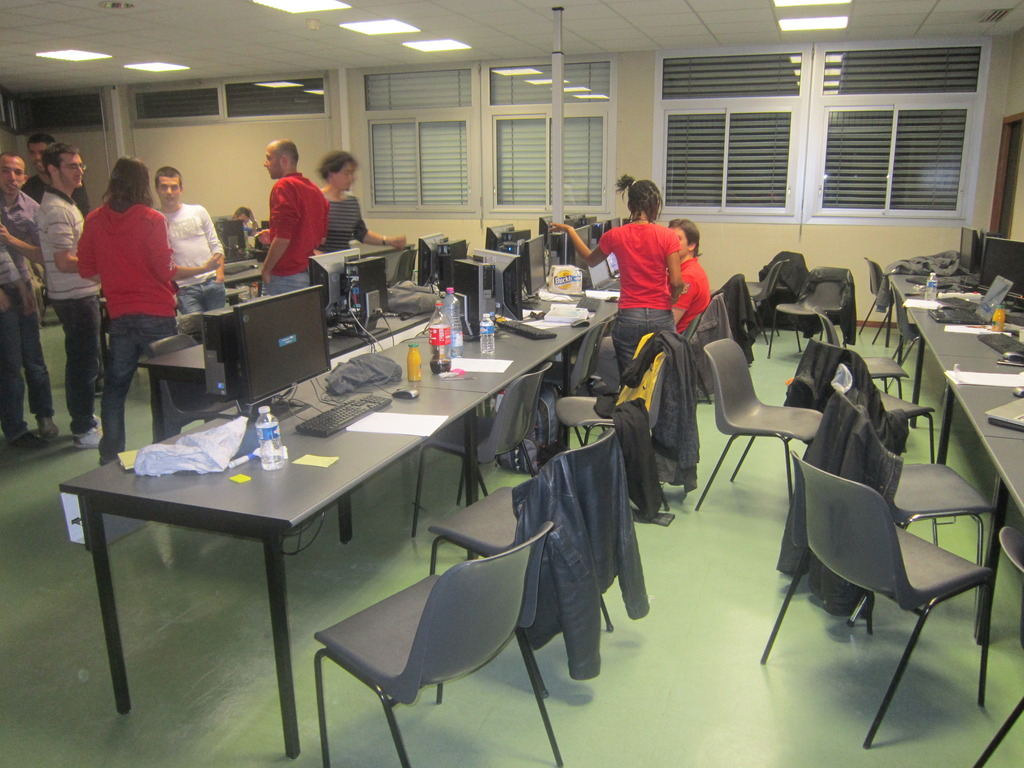
\includegraphics[scale=0.38]{brainstorming3.jpeg} \\
    Les défis méritaient parfois des mises aux points. \\
    
    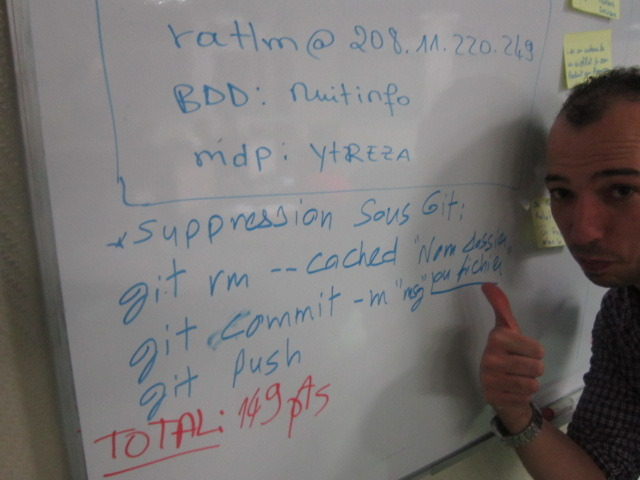
\includegraphics[scale=0.6]{gi.jpeg} \hspace{0.3cm} 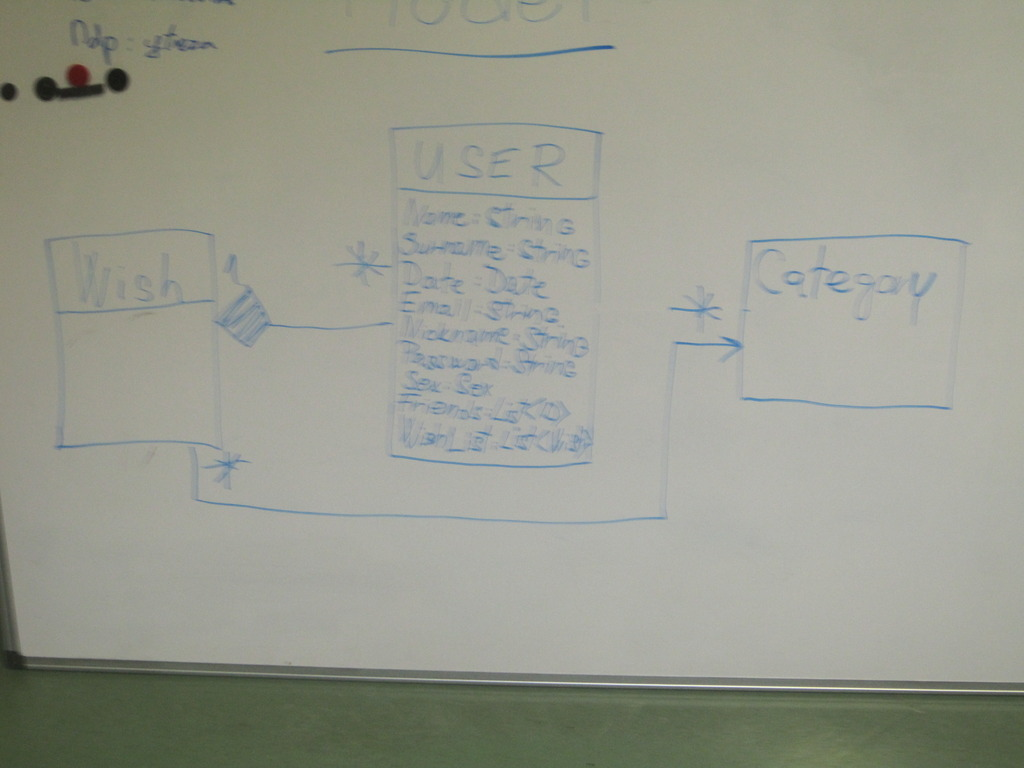
\includegraphics[scale=0.378]{shema.jpeg} \\
    
    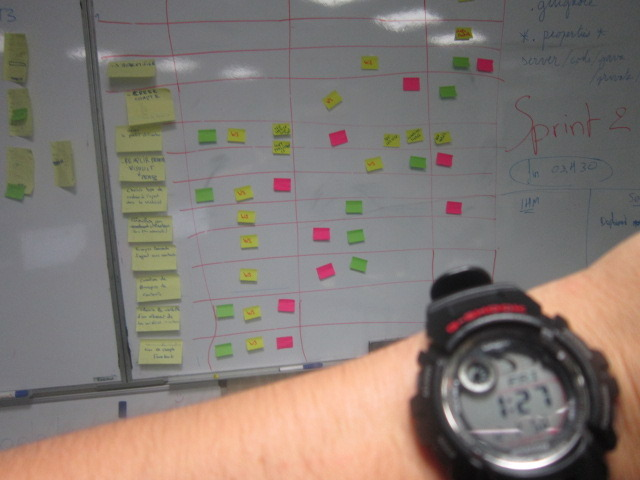
\includegraphics[scale=0.6]{sprint.jpeg} \hspace{0.3cm} \includegraphics[scale=0.06]{tache.jpg} \\
    Le tableau a joué un élément principal dans la méthodologie, pour véhiculer des informations et prendre les tâches. \\
 
\pagebreak   
\section{Bilan}
  Au final nous avons bien réussi à appliquer la méthode SCRUM, chacun jouant le jeu, mais nous nous sommes heurté à des problèmes techniques de plus en plus compliqués qui au final nous ont bloqué dans la finalisation du projet. Cependant cette expérience d'extrême programming concentré a quand même été une bonne chose. L'une des leçons que nous tirerons de cette nuit est de toujours penser au plus simple, et de ne pas utiliser un objet non créé...

\end{document}	